% Midterm presentation — COMP-SCI 5567 Group 4
% Build:  latexmk -pdf midterm.tex     (or let CI do it)
\documentclass[aspectratio=169,11pt]{beamer}

\usetheme{metropolis}
\usepackage{booktabs}
\usepackage{tikz}
\usetikzlibrary{arrows.meta, positioning, shapes.geometric, fit, backgrounds, calc}
\usepackage{xcolor}

\definecolor{umkcblue}{HTML}{005583}
\definecolor{accent}{HTML}{E08B2E}
\definecolor{ok}{HTML}{2E8B57}
\setbeamercolor{frametitle}{bg=umkcblue}
\setbeamercolor{progress bar}{fg=accent}

\title{Video Object Tracking on MOT16}
\subtitle{Faster R-CNN detection with Siamese re-identification}
\author{Ben Blake \and Geethika Padamati \and Tina Nguyen \and Sanjana Aileni}
\institute{Group 4 \\ COMP-SCI 5567 --- Deep Learning \\ University of Missouri--Kansas City}
\date{Midterm Presentation}

% Pipeline box styles, reused across diagrams.
\tikzset{
  stage/.style={rectangle, rounded corners=3pt, draw=umkcblue, fill=umkcblue!8,
                text width=2.5cm, align=center, minimum height=1.1cm, font=\small},
  io/.style={rectangle, rounded corners=3pt, draw=gray!60, fill=gray!10,
             text width=2.1cm, align=center, minimum height=1.0cm, font=\small},
  flow/.style={-{Stealth[length=2.5mm]}, thick, draw=gray!70},
}

\begin{document}

\maketitle

% ─────────────────────────────────────────────── Ben: problem and system
\begin{frame}{The team and the split}
  \begin{columns}[T,onlytextwidth]
    \column{0.5\textwidth}
      \textbf{Ben Blake} --- detection \& tracking \\
      {\small Faster R-CNN, data association, integration}
      \vspace{0.6em}

      \textbf{Geethika Padamati} --- data pipeline \\
      {\small MOT16 parsing, datasets, augmentation}
    \column{0.5\textwidth}
      \textbf{Tina Nguyen} --- re-identification \\
      {\small Siamese network, contrastive loss}
      \vspace{0.6em}

      \textbf{Sanjana Aileni} --- evaluation \& demo \\
      {\small Metrics, visualization, result video}
  \end{columns}
  \vspace{1.2em}
  \hrule
  \vspace{0.8em}
  Each of us owns one module end to end --- its code, its slides, its section of
  the report.
\end{frame}

\begin{frame}{The problem}
  \textbf{Given} a video, \textbf{produce} a box around each pedestrian in every
  frame, with the \alert{same identity number} following the same person.
  \vspace{1em}

  \begin{columns}[T,onlytextwidth]
    \column{0.5\textwidth}
      \textbf{Detection alone is not enough}

      A detector answers \emph{``where are the people?''} independently in each
      frame. It has no notion that the person in frame 10 is the person from
      frame 9.
    \column{0.5\textwidth}
      \textbf{Tracking adds identity over time}

      We must link detections across frames --- through occlusion, through
      people crossing, through the detector missing a frame entirely.
  \end{columns}
  \vspace{1em}
  \begin{alertblock}{Target (course rubric)}
    Track at least one target pedestrian across an MOT16 test sequence without
    losing it.
  \end{alertblock}
\end{frame}

\begin{frame}{Why this matters}
  \begin{columns}[T,onlytextwidth]
    \column{0.52\textwidth}
      \begin{itemize}
        \item \textbf{Autonomous driving} --- a pedestrian that changes ID is a
              pedestrian whose trajectory you cannot predict
        \item \textbf{Surveillance and safety} --- counting, flow, anomalies
        \item \textbf{Sports analytics} --- per-player statistics require
              per-player identity
        \item \textbf{Retail and robotics} --- movement patterns, navigation
      \end{itemize}
    \column{0.44\textwidth}
      \begin{block}{The common thread}
        Every application needs \emph{identity}, not just location. Knowing
        \emph{someone} is at a position is rarely enough --- you need to know
        \emph{who}, and for how long.
      \end{block}
  \end{columns}
\end{frame}

\begin{frame}{System architecture}
  \centering
  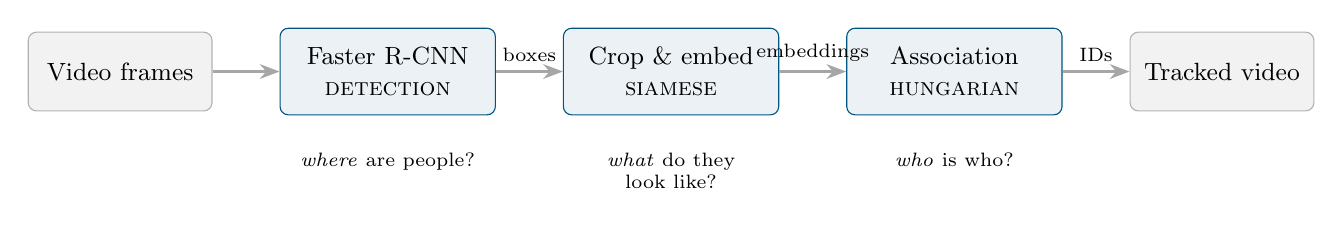
\begin{tikzpicture}[node distance=0.85cm]
    \node[io] (frames) {Video frames};
    \node[stage, right=of frames] (detect) {Faster R-CNN\\\textsc{detection}};
    \node[stage, right=of detect] (crop) {Crop \& embed\\\textsc{siamese}};
    \node[stage, right=of crop] (assoc) {Association\\\textsc{hungarian}};
    \node[io, right=of assoc] (out) {Tracked video};

    \draw[flow] (frames) -- (detect);
    \draw[flow] (detect) -- node[above, font=\scriptsize] {boxes} (crop);
    \draw[flow] (crop) -- node[above, font=\scriptsize] {embeddings} (assoc);
    \draw[flow] (assoc) -- node[above, font=\scriptsize] {IDs} (out);

    \node[below=0.35cm of detect, font=\scriptsize, text width=2.6cm, align=center]
      {\emph{where} are people?};
    \node[below=0.35cm of crop, font=\scriptsize, text width=2.6cm, align=center]
      {\emph{what} do they look like?};
    \node[below=0.35cm of assoc, font=\scriptsize, text width=2.6cm, align=center]
      {\emph{who} is who?};
  \end{tikzpicture}
  \vspace{1.2em}

  \begin{columns}[T,onlytextwidth]
    \column{0.48\textwidth}
      \textbf{Offline tracking.} We process a batch of frames rather than
      streaming, which lets us recover from short occlusions.
    \column{0.48\textwidth}
      \textbf{Tracking by detection.} Detection and identity are separate
      problems; separating them lets us swap either component independently.
    \end{columns}
\end{frame}

\begin{frame}{Detection: Faster R-CNN}
  \begin{columns}[T,onlytextwidth]
    \column{0.55\textwidth}
      \textbf{Why this model}
      \begin{itemize}
        \item Region Proposal Network makes proposals \emph{inside} the network
              --- no external Selective Search
        \item Proposals and detection share one backbone, so the image is
              convolved once
        \item Accurate on small objects --- distant pedestrians are small
      \end{itemize}
      \vspace{0.5em}
      \textbf{Few-shot fine-tuning}

      We freeze the ResNet50-FPN backbone and train only the heads, as the
      assignment suggests.
    \column{0.42\textwidth}
      \begin{block}{Parameter budget}
        \begin{tabular}{lr}
          \toprule
          Total      & 41.3\,M \\
          Frozen     & 26.8\,M \\
          \textbf{Trainable} & \textbf{14.5\,M} \\
          \bottomrule
        \end{tabular}
        \vspace{0.4em}

        {\footnotesize 35\% trainable --- fits comfortably in Colab's VRAM.}
      \end{block}
  \end{columns}
\end{frame}

\begin{frame}{The association problem}
  Each frame gives $N$ detections; we hold $M$ existing tracks. Which detection
  continues which track?
  \vspace{0.8em}

  \begin{columns}[T,onlytextwidth]
    \column{0.47\textwidth}
      \textbf{Overlap alone fails}

      When two people cross, their boxes overlap each other's previous
      position. Position cannot tell them apart.
      \vspace{0.6em}

      \textbf{Appearance alone fails}

      Two people in similar clothing look alike. Appearance drifts.
    \column{0.49\textwidth}
      \begin{block}{Blended cost}
        \[
          C_{ij} = (1-\lambda)\underbrace{(1 - \mathrm{IoU}_{ij})}_{\text{where}}
                 + \lambda \underbrace{(1 - \cos(e_i, e_j))}_{\text{what}}
        \]
        Solved with the Hungarian algorithm for a globally optimal one-to-one
        assignment. Pairs failing either gate are forbidden outright.
      \end{block}
  \end{columns}
  \vspace{0.5em}
  {\footnotesize A track survives \texttt{max\_age} unmatched frames, so a brief
  occlusion does not spawn a new identity.}
\end{frame}

% ─────────────────────────────────────────────── Geethika: data
\begin{frame}{The MOT16 dataset}
  \begin{columns}[T,onlytextwidth]
    \column{0.5\textwidth}
      \begin{itemize}
        \item 14 sequences --- 7 train (with ground truth), 7 test
        \item Crowded streets, moving and static cameras
        \item Heavy occlusion; people leave and re-enter frame
      \end{itemize}
      \vspace{0.6em}
      \textbf{One annotation row}
      \vspace{0.3em}

      {\footnotesize\texttt{1, 3, 586, 447, 85, 263, 1, 1, 1}}
    \column{0.47\textwidth}
      \begin{block}{Columns}
        {\footnotesize
        \begin{tabular}{ll}
          \texttt{frame}      & 1 \\
          \texttt{id}         & 3 \\
          \texttt{bb\_left}   & 586 \\
          \texttt{bb\_top}    & 447 \\
          \texttt{bb\_width}  & 85 \\
          \texttt{bb\_height} & 263 \\
          \texttt{conf}       & 1 (0 = ignore) \\
          \texttt{class}      & 1 (pedestrian) \\
          \texttt{visibility} & 1.0 \\
        \end{tabular}}
      \end{block}
  \end{columns}
\end{frame}

\begin{frame}{Two traps in the annotations}
  \begin{columns}[T,onlytextwidth]
    \column{0.48\textwidth}
      \begin{alertblock}{Coordinates are 1-indexed}
        The files count pixels from 1; NumPy counts from 0. Ignoring this
        shifts every box by one pixel --- small enough to pass review, large
        enough to quietly cost IoU.
      \end{alertblock}
    \column{0.48\textwidth}
      \begin{alertblock}{Not every person is a target}
        Class 7 (static person), 8 (distractor) and 12 (reflection) are people
        but are \emph{not} scored. Training on them teaches the detector to
        fire on mannequins and mirrors.
      \end{alertblock}
  \end{columns}
  \vspace{1em}
  Both are handled in \texttt{mot/data/mot16.py} and covered by unit tests ---
  these are exactly the bugs that are invisible until the metrics are
  inexplicably bad.
\end{frame}

\begin{frame}{Data augmentation}
  \begin{columns}[T,onlytextwidth]
    \column{0.5\textwidth}
      A handful of scenes means the real risk is \emph{memorising those scenes}
      rather than learning what a pedestrian looks like.
      \vspace{0.6em}

      \textbf{Detection}
      \begin{itemize}
        \item Horizontal flip (boxes mirrored with the image)
        \item Colour jitter --- brightness, contrast, saturation
      \end{itemize}
      \vspace{0.4em}
      \textbf{Re-ID crops}
      \begin{itemize}
        \item Random crop and flip
        \item Random erasing --- simulated occlusion
      \end{itemize}
    \column{0.46\textwidth}
      \begin{block}{What we deliberately do \emph{not} do}
        No vertical flips or large rotations. Pedestrians are upright in every
        frame of every sequence; training on upside-down people teaches a pose
        the model will never encounter and wastes capacity.
      \end{block}
  \end{columns}
\end{frame}

% ─────────────────────────────────────────────── Tina: re-identification
\begin{frame}{Re-identification}
  \textbf{The question:} do these two crops, from different frames, show the
  same person?
  \vspace{0.8em}

  \begin{columns}[T,onlytextwidth]
    \column{0.47\textwidth}
      \begin{block}{Naive approach: classification}
        Train a classifier over the people in the video.

        \alert{Fails:} every new person entering the scene requires retraining,
        and MOT16 sequences are full of people entering.
      \end{block}
    \column{0.49\textwidth}
      \begin{block}{Our approach: a similarity model}
        Learn an \emph{embedding} where the same person lands close together
        and different people land far apart.

        \textbf{Never needs retraining} for new people --- it learned
        similarity, not a fixed list of identities.
      \end{block}
  \end{columns}
\end{frame}

\begin{frame}{Siamese network}
  \centering
  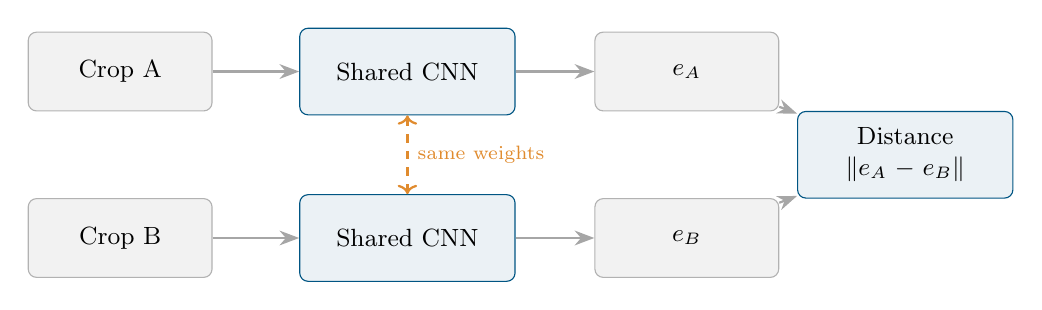
\begin{tikzpicture}[node distance=0.7cm]
    \node[io] (a) {Crop A};
    \node[io, below=1.1cm of a] (b) {Crop B};
    \node[stage, right=1.1cm of a] (cnna) {Shared CNN};
    \node[stage, right=1.1cm of b] (cnnb) {Shared CNN};
    \node[io, right=1.0cm of cnna] (ea) {$e_A$};
    \node[io, right=1.0cm of cnnb] (eb) {$e_B$};
    \node[stage, right=1.4cm of $(ea)!0.5!(eb)$] (d) {Distance\\$\Vert e_A - e_B\Vert$};

    \draw[flow] (a) -- (cnna);
    \draw[flow] (b) -- (cnnb);
    \draw[flow] (cnna) -- (ea);
    \draw[flow] (cnnb) -- (eb);
    \draw[flow] (ea) -- (d);
    \draw[flow] (eb) -- (d);
    \draw[<->, dashed, thick, accent] (cnna) -- node[right, font=\scriptsize] {same weights} (cnnb);
  \end{tikzpicture}
  \vspace{0.8em}

  \begin{columns}[T,onlytextwidth]
    \column{0.46\textwidth}
      {\footnotesize
      4 conv blocks $\rightarrow$ adaptive pool $\rightarrow$ 128-d embedding,
      L2-normalised. 1.5\,M parameters --- small enough to train in minutes.}
    \column{0.50\textwidth}
      \begin{block}{Contrastive loss}
        \vspace{-0.6em}
        \[
          L = \tfrac12\left[ y\,d^2 + (1-y)\max(0, m - d)^2 \right]
        \]
        \vspace{-0.8em}

        {\footnotesize Pull matching pairs together; push different pairs apart
        past margin $m$.}
      \end{block}
  \end{columns}
\end{frame}

\begin{frame}{A problem we had to resolve}
  \begin{alertblock}{The course slides contradict themselves on crop size}
    Training is specified at $16\times16$, inference at $24\times24$, retrieved
    crops at $30\times16$ --- and the reference \texttt{Siamese\_Network} code
    has \texttt{nn.Linear(128 * 22 * 22, ...)}, which actually requires a
    ${\sim}102\times102$ input. No single size satisfies all four.
  \end{alertblock}
  \vspace{0.5em}

  \begin{columns}[T,onlytextwidth]
    \column{0.48\textwidth}
      \textbf{What we chose}
      \begin{itemize}
        \item $128\times64$ --- the standard person Re-ID aspect ratio, matching
              Market-1501
        \item \texttt{AdaptiveAvgPool2d} instead of a hardcoded flatten
      \end{itemize}
    \column{0.48\textwidth}
      \textbf{Why}
      \begin{itemize}
        \item $16\times16$ cannot resolve clothing detail --- the entire signal
              Re-ID depends on
        \item Adaptive pooling makes the network accept \emph{any} input size,
              so the contradiction cannot bite us again
      \end{itemize}
  \end{columns}
\end{frame}

% ─────────────────────────────────────────────── Sanjana: evaluation and demo
\begin{frame}{How we measure success}
  \begin{columns}[T,onlytextwidth]
    \column{0.52\textwidth}
      \begin{block}{CLEAR-MOT metrics}
        \vspace{-0.4em}
        \[ \mathrm{MOTA} = 1 - \frac{\mathrm{FN} + \mathrm{FP} + \mathrm{IDSW}}{\text{ground truth}} \]
        \vspace{-0.6em}
        \begin{itemize}\footnotesize
          \item \textbf{FN} --- a person we missed
          \item \textbf{FP} --- a box with nobody in it
          \item \textbf{IDSW} --- the ID changed on the same person
        \end{itemize}
      \end{block}
      \vspace{-0.3em}
      {\footnotesize \textbf{MOTP} --- mean IoU of matched boxes: how
      \emph{tight} the boxes are.}
    \column{0.44\textwidth}
      \begin{block}{Why ID switches matter most}
        A missed frame is recoverable. An ID switch means we have
        \emph{confused two people} --- the one failure the whole Re-ID component
        exists to prevent, and the one the rubric grades.
      \end{block}
  \end{columns}
\end{frame}

\begin{frame}{Where we are}
  \begin{columns}[T,onlytextwidth]
    \column{0.52\textwidth}
      \textbf{Working today}
      \begin{itemize}
        \item[\textcolor{ok}{\textbullet}] Full pipeline runs end to end
        \item[\textcolor{ok}{\textbullet}] MOT16 parsing, 1-indexing and
              ignore-classes handled
        \item[\textcolor{ok}{\textbullet}] Siamese network trains and converges
        \item[\textcolor{ok}{\textbullet}] Tracker survives occlusion; IDs stable
        \item[\textcolor{ok}{\textbullet}] MOTA/MOTP/IDSW implemented
        \item[\textcolor{ok}{\textbullet}] 36 unit tests, green in CI
      \end{itemize}
    \column{0.44\textwidth}
      \textbf{Next}
      \begin{itemize}
        \item Fine-tune the detector on MOT16
        \item Train Re-ID on Market-1501 + MOT16 crops
        \item Sweep $\lambda$, IoU and age thresholds
        \item Ablation: with vs.\ without Re-ID
        \item Final video on a test sequence
      \end{itemize}
  \end{columns}
  \vspace{0.6em}
  \hrule
  \vspace{0.5em}
  {\footnotesize Baseline uses the COCO-pretrained detector, so the system
  produced tracked video \emph{before} any training --- fine-tuning is an
  improvement, not a prerequisite.}
\end{frame}

\begin{frame}[standout]
  Demo
\end{frame}

\begin{frame}{Timeline to the final}
  \centering
  \begin{tabular}{lll}
    \toprule
    \textbf{Phase} & \textbf{Work} & \textbf{Owner} \\
    \midrule
    Done          & Pipeline, parsing, Re-ID, metrics, CI & All \\
    Midterm week  & Baseline run, demo recorded           & Sanjana \\
    Next          & Detector fine-tuning                  & Ben \\
    Next          & Re-ID training on real data           & Tina \\
    Next          & Augmentation tuning                   & Geethika \\
    Then          & Threshold sweep, ablations            & Sanjana, Ben \\
    Final         & Report, final video, presentation     & All \\
    \bottomrule
  \end{tabular}
  \vspace{1.2em}

  {\footnotesize Code: \texttt{github.com/ben-blake/cs5567-project}}
\end{frame}

\begin{frame}[standout]
  Questions
\end{frame}

\end{document}
